\section{Scenario 4}\label{sec:scenario4}
The purpose of this scenario is to show what can happen when the UAS loses line-of-sight, because of a mountain as seen on the map in Figure \ref{fig:s4_map}. Also, the controller used in the simulation is a PD controller.

\begin{figure}[H]
\hfill
\subfigure[UAS Map Positioning]{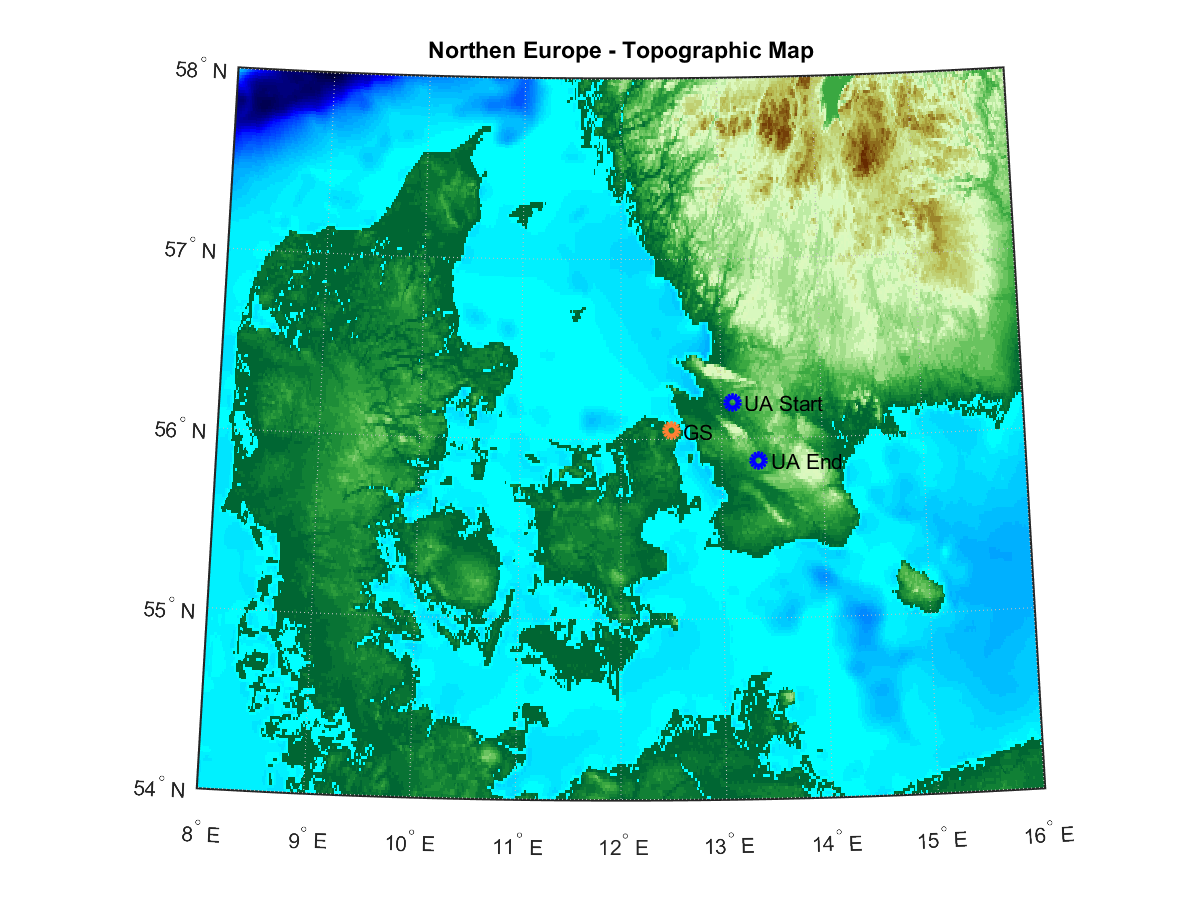
\includegraphics[scale=0.33]{figures/scenario_4_map.png}}
\hfill
\subfigure[LOS and Distance]{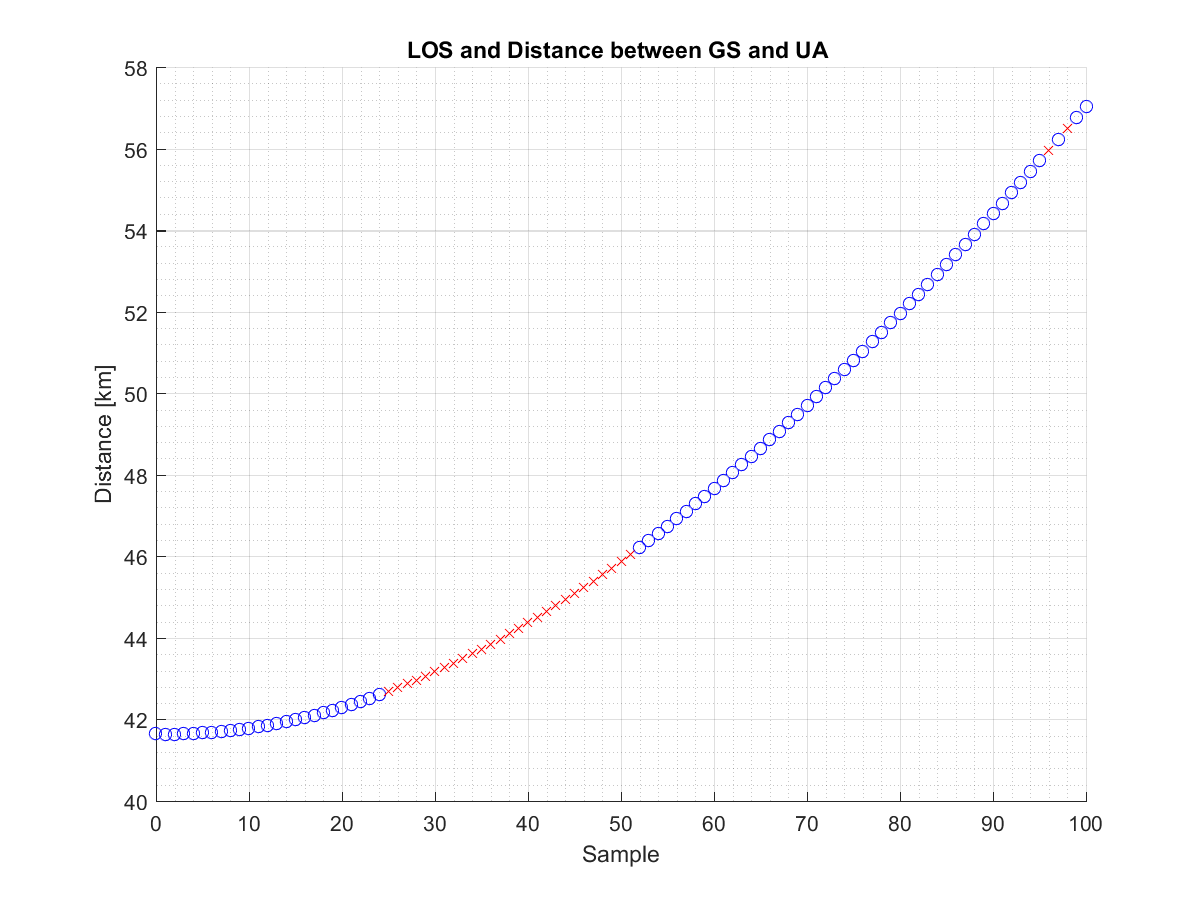
\includegraphics[scale=0.33]{figures/scenario_4_los.png}}
\hfill
\caption{Mountain Scenario}
\label{fig:s4_map}
\end{figure}

\subsection{UA}


\begin{figure}[H]
\begin{minipage}[t]{0.45\textwidth}
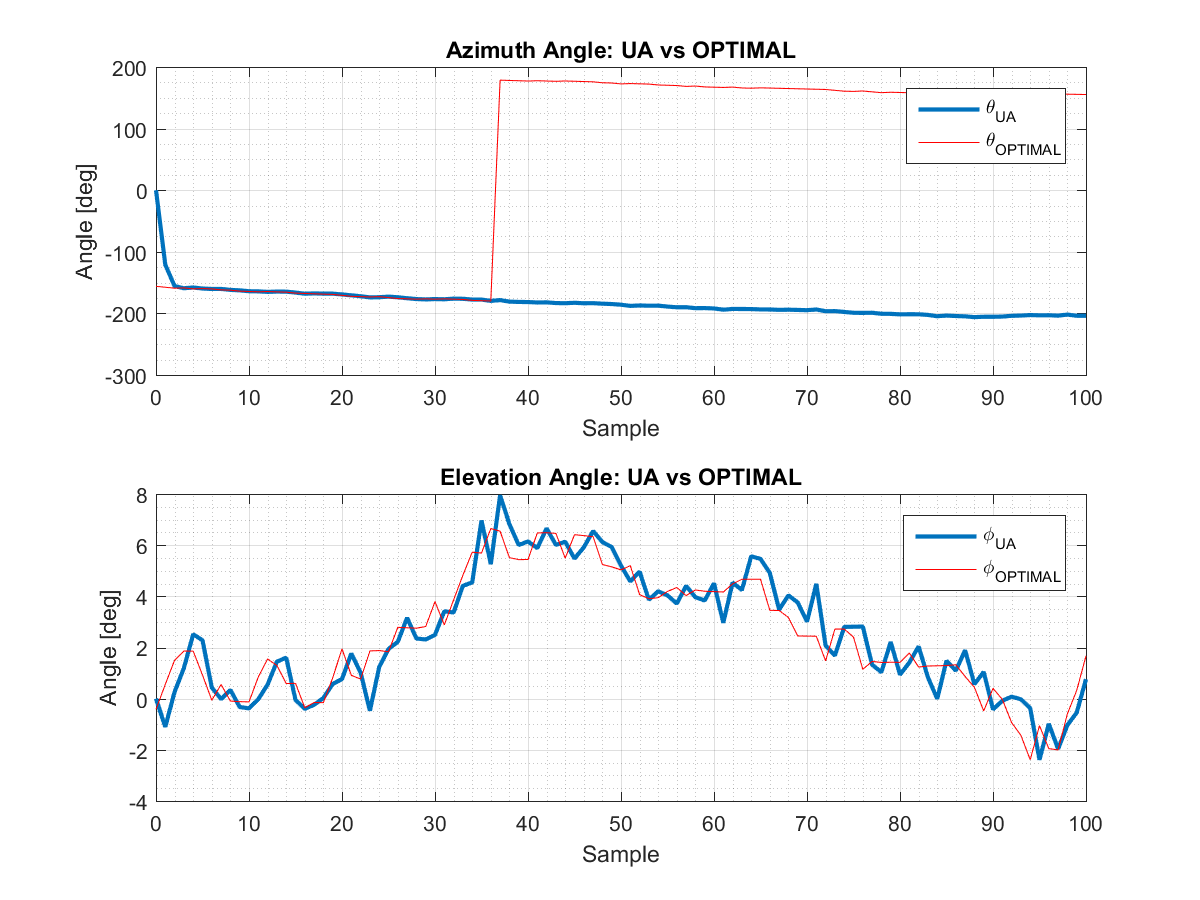
\includegraphics[width=\linewidth]{figures/scenario_4_ua.png}
\caption{p}
\label{fig:s1_drones_p}
\end{figure}

\subsection{GS}


\begin{figure}[H]
\begin{minipage}[t]{0.45\textwidth}
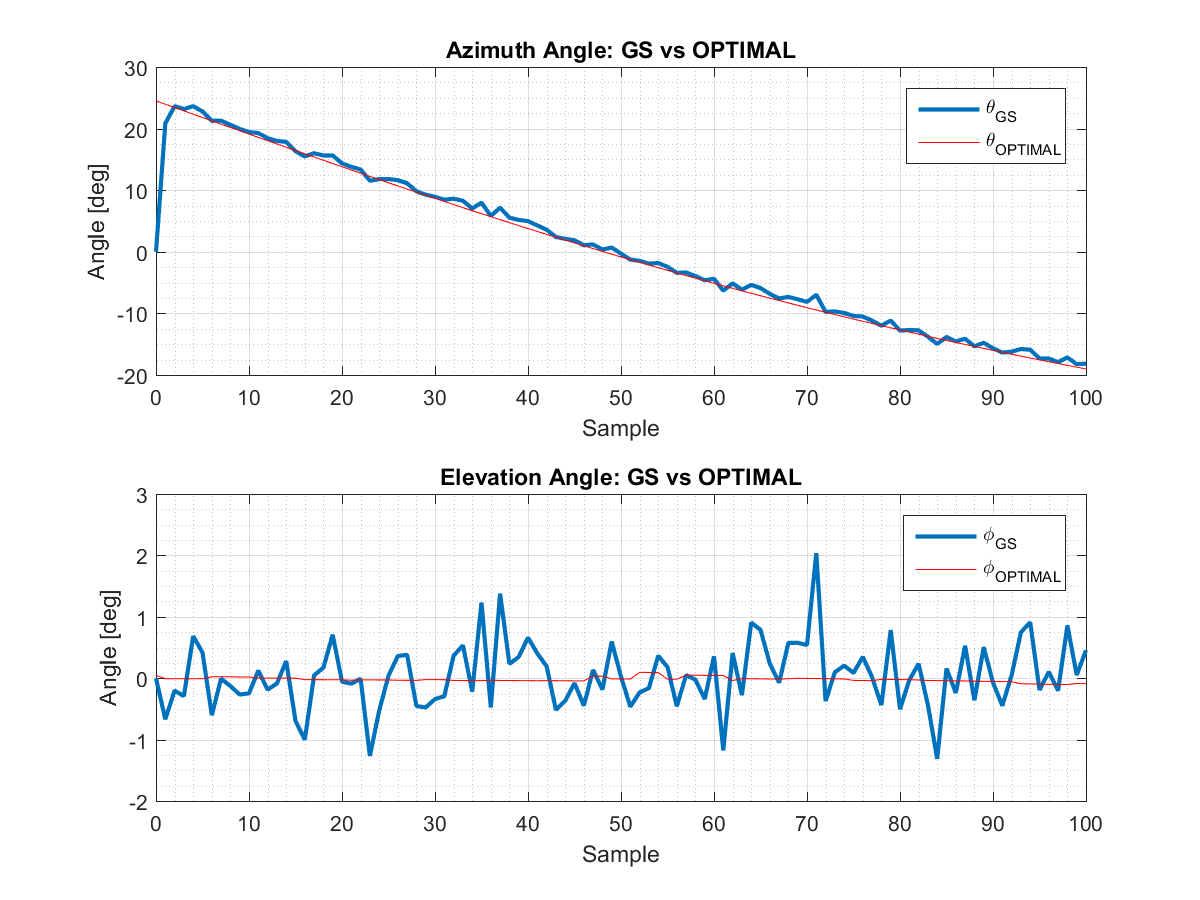
\includegraphics[width=\linewidth]{figures/scenario_4_gs.png}
\caption{p}
\label{fig:s1_drones_p}
\end{figure}

\subsection{Power}


\begin{figure}[H]
\begin{minipage}[t]{0.45\textwidth}
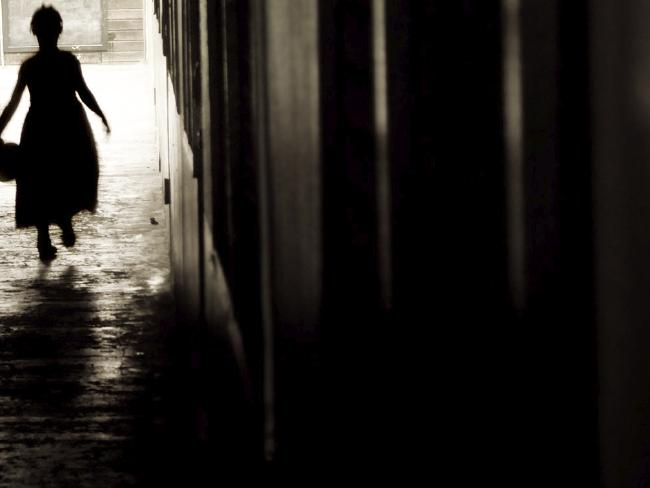
\includegraphics[width=\linewidth]{figures/randomfigure.jpg}
\caption{p}
\label{fig:s1_drones_p}
\end{figure}